\documentclass[a4paper,11pt]{article}
\usepackage{polski}
\usepackage[utf8]{inputenc}

% \usepackage{a4wide}

\usepackage{amsmath}
\usepackage{amsfonts}
% \usepackage{amssymb}
% \usepackage{amsthm}
\usepackage{listings}
\usepackage{graphicx}

\title{
  \textbf{Pracownia 02}\\
  {\Large Podstawy elektroniki, elektrotechniki i miernictwa}
}
\author{Rafał Łasocha}
\setcounter{equation}{0}

\begin{document}

\maketitle

\section{Zagadnienia teoretyczne}

\subsection{Oscyloskop}
Oscyloskop jest przyrządem elektronicznym służącym do obserwowania wykresów zależności pomiędzy wartością napięcia a czasem. Mamy również możliwość pomiaru różnych wartości (amplitudy, częstotliwości). Na zajęciach korzystaliśmy z oscyloskopu cyfrowego PeakTech 1200 oraz oscyloskopu analogowego.

\subsection{Układ całkujący}
Układ, którego funkcja napięcia wyjściowego może być przedstawiona wzorem:
$$
y(t) = \int_{-\inf}^t u(\tau) \mathtt{d}\tau
$$
gdzie $u(\tau)$ to funkcja sygnału wejściowego. Przedstawiony na rysunku 1.

\begin{figure}[h]
 \begin{center}
  
\includegraphics[width=8cm]{uklad_calkujacy}
 \end{center}
 \caption{Układ całkujący}
\end{figure}

\subsection{Układ różniczkujący}
Układ, którego napięcie wyjściowe jest proporcjonalne do szybkości zmian napięcia wejściowego. Układ różniczkujący może być zbudowany jako pasywny albo aktywny, na zajęciach korzystaliśmy z układu aktywnego, który zbudowany jest tak jak na rysunku 2.

\begin{figure}[h]
 \begin{center}
  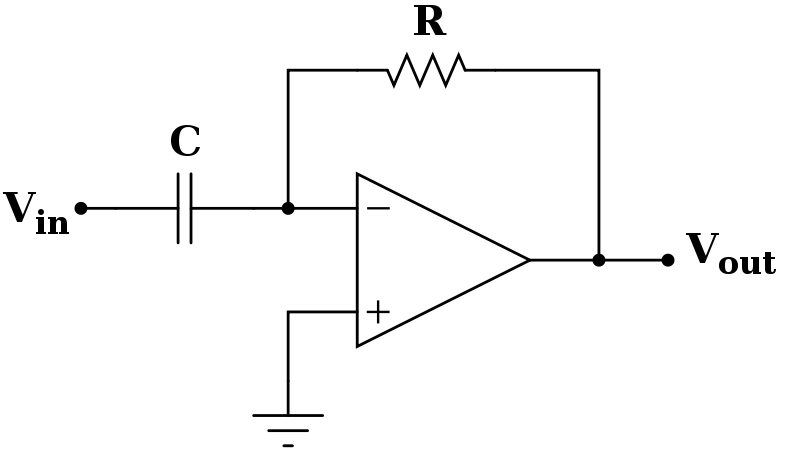
\includegraphics[width=8cm]{uklad_rozniczkujacy}
 \end{center}
 \caption{Układ różniczkujący}
\end{figure}

\subsection{Prostownik}
Układ, który zamienia napięcie przemienne na napięcie tylko jednego znaku.



\section{Przebieg ćwiczenia}
Na początku podłączyliśmy generator akustyczny z częstotliwością 1kHz. Amplituda sygnału wynosiła 1.8V, a sam sygnał wyglądał tak jak na rysunku 3.

\begin{figure}[h]
 \begin{center}
  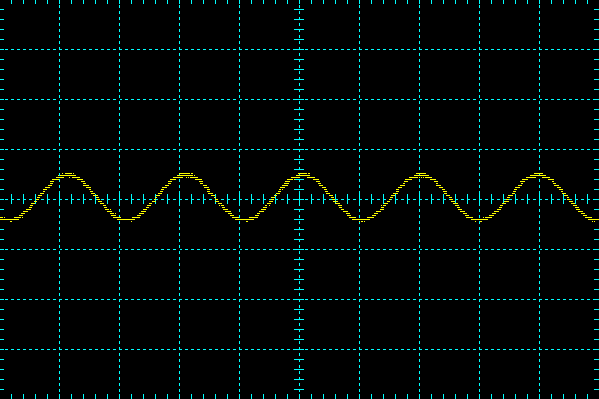
\includegraphics[width=12cm]{gen_akustyczny}
 \end{center}
 \caption{Wykres sygnału z częstotliwością 1kHz}
\end{figure}

Próba odczytania wyniku z oscyloskopu analogowego dała nam wynik 1087Hz.

Następnie podłączyliśmy generator akustyczny przez opornik 1M$\Omega$. Amplituda sygnały wynosiła 340mV, a sygnał jest przedstawiony na rysunku 4.

\begin{figure}[h]
 \begin{center}
  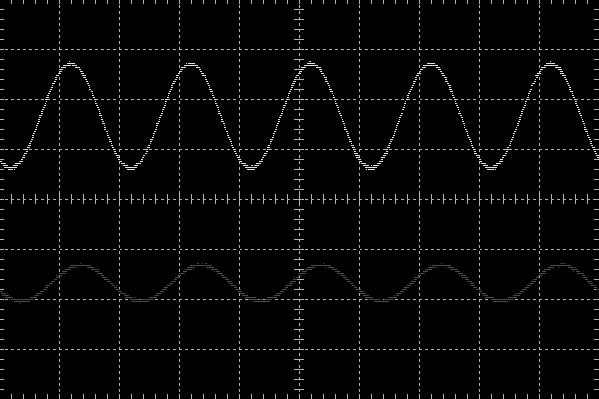
\includegraphics[width=12cm]{gen_akustyczny_z_opornikiem}
 \end{center}
 \caption{Wykres sygnału z częstotliwością 1kHz i opornikiem}
\end{figure}

Drugim etapem ćwiczenia było podłączenie prostownika w różnych kombinacjach opornika i kondensatora.

Dla prostownika przeprowadziliśmy trzy próby: z pojemnością 1C i 1R, 1C i 4R, 10C i 1R, oraz 10C i 4R, gdzie $1C = 4.7\mu F$ oraz $1R = 0.5K\Omega$, aby zaobserwować jakie zmiany zachodzą w wykresach sygnału. Wykresy sygnału są pokazane na rysunkach 5, 6, 7 i 8. Amplitudy sygnału wynosiły kolejno: 16V, 10V, 4.5V oraz 2V.

\begin{figure}[ht]
 \begin{center}
  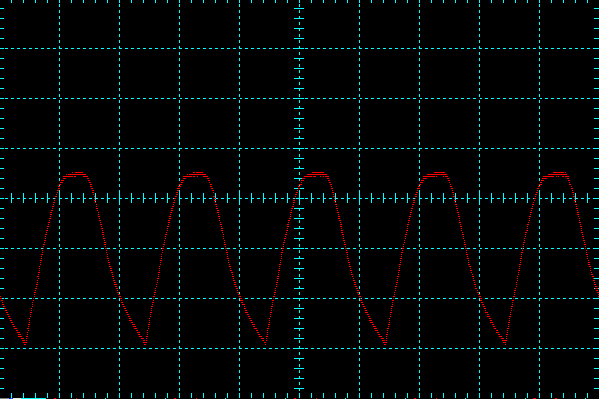
\includegraphics[width=12cm]{prostownik_1C_1R}
 \end{center}
 \caption{Prostownik, kondensator 1C, opornik 1R}
\end{figure}

\begin{figure}[ht]
 \begin{center}
  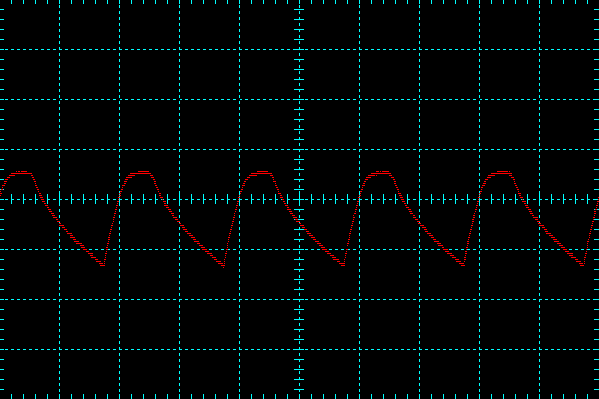
\includegraphics[width=12cm]{prostownik_1C_4R}
 \end{center}
 \caption{Prostownik, kondensator 1C, opornik 4R}
\end{figure}

\begin{figure}[ht]
 \begin{center}
  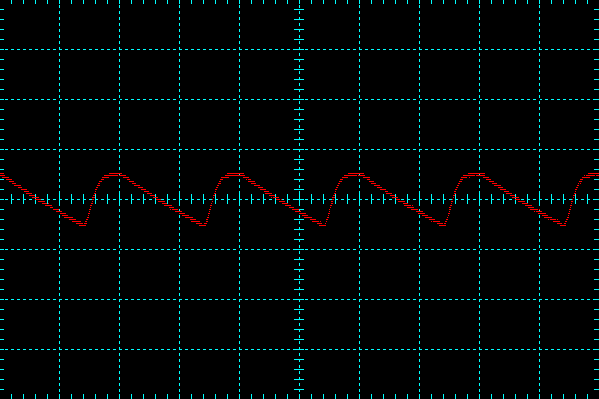
\includegraphics[width=12cm]{prostownik_10C_1R}
 \end{center}
 \caption{Prostownik, kondensator 10C, opornik 1R}
\end{figure}

\begin{figure}[ht]
 \begin{center}
  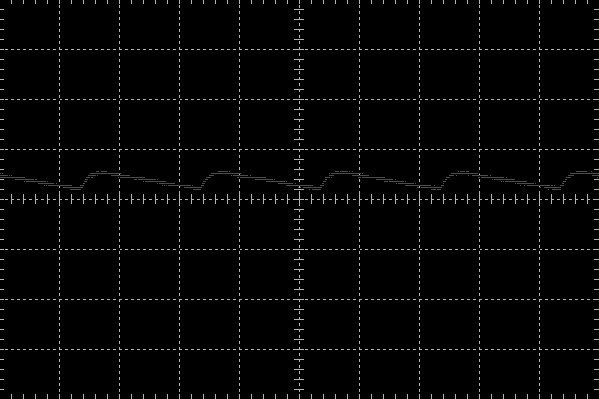
\includegraphics[width=12cm]{prostownik_10C_4R}
 \end{center}
 \caption{Prostownik, kondensator 10C, opornik 4R}
\end{figure}

Następnie podłączyliśmy dwa układy, pierwszym z nich był układ różniczkujący. Podłączyliśmy go na dwa sposoby, raz z pojemnością 5C i oporem 1R, a drugi raz z pojemnością 25C i oporem 0.5R. Wykresy sygnału przedstawiają rysunki 9 i 10.

\begin{figure}[ht]
 \begin{center}
  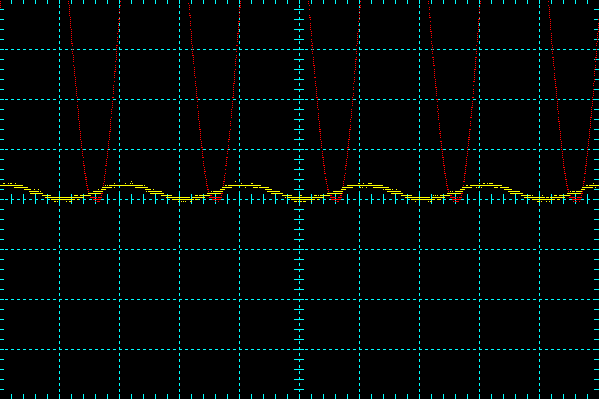
\includegraphics[width=12cm]{rozniczkujacy_5C_1R}
 \end{center}
 \caption{Układ różniczkujący, kondensator 5C, opornik 1R}
\end{figure}

\begin{figure}[ht]
 \begin{center}
  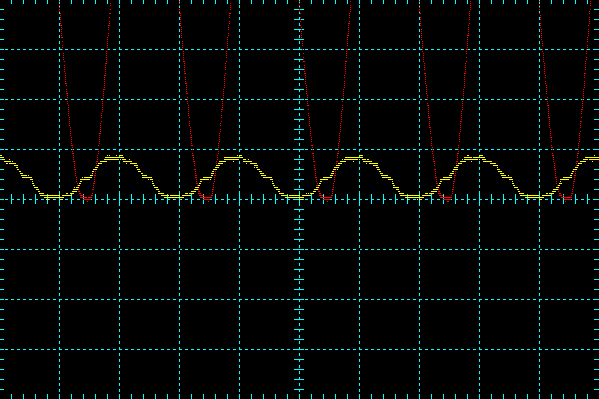
\includegraphics[width=12cm]{rozniczkujacy_25C_05R}
 \end{center}
 \caption{Układ różniczkujący, kondensator 25C, opornik 0.5R}
\end{figure}

Ostatnią częścią było podłączenie układu całkującego, wykonaliśmy to z pojemnością 0.1C i oporem 1R. Wykres sygnału przedstawia rysunek 11.

\begin{figure}[ht]
 \begin{center}
  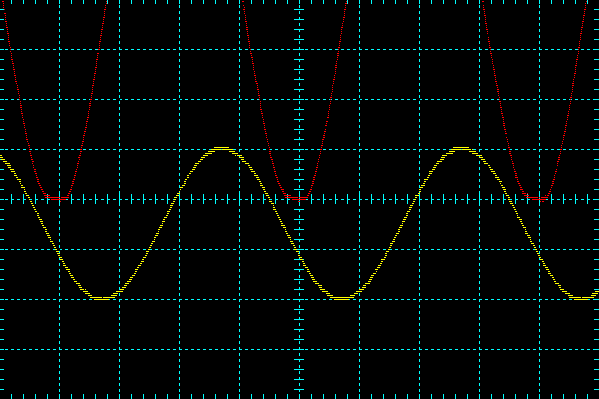
\includegraphics[width=12cm]{calkujacy_1R_01C}
 \end{center}
 \caption{Układ całkujący, kondensator 0.1C, opornik 1R}
\end{figure}


\section{Wnioski}
Pierwsze dwa wykresy przedstawiają podłączenie generatora akustycznego bez opornika oraz z opornikiem. Po podłączeniu opornika, spadła amplituda, co było spodziewanym efektem. Dowiedzieliśmy się też, że oscyloskopem analogowym ciężej zmierzyć dokładne wartości (amplitudy), ponieważ otrzymaliśmy wynik o 8.7\% większy od wyniku z oscyloskopu cyfrowego.
Druga część ćwiczenia z podłączaniem prostownika pokazała nam jak dobór kondensatora i opornika w prostowniku ma wpływ na wykres sygnału.
W ostatniej części podłączyliśmy układ całkujący i różniczkujący. Próbowaliśmy różne konfiguracje i układy przedstawiały oczekiwany wynik.


\end{document}